\documentclass[12pt, oneside]{article}

\usepackage{./texmf/preamble}

\graphicspath{{./assets/}}
\addglobalbib{sources.bib}

\onehalfspacing

\immediate\write18{texcount -merge \jobname.tex | sed -n 's/.*Words in text://p' | awk '{$1=$1};1' > 'count.txt'}

\providecommand{\totalwordcount}{\input{count.txt}}

% =================================================================
% Content
% =================================================================

\begin{document} % BEGIN
\pagestyle{frontmatter}

\begin{titlepage}
    \large

    \begin{center}

        \vspace*{2cm}

        {\bfseries
            IB Math Analysis and Approaches (HL) \\
            Extended Essay\\
            May 2024 Session}\\

        \vspace*{\fill}

        \rule{\linewidth}{1.5pt} \\ [0.5cm]
        {\LARGE \bfseries Mathematical Techniques and Applications of Camera Calibration }
        \rule{\linewidth}{0.5pt} \\

        \vspace*{\fill}

        \textbf{Research Question:} What mathematical techniques can be employed to develop highly accurate camera models, and what are their real-world applications where these models prove valuable? \\ [1cm]

        \textbf{Word Count:} \totalwordcount words

        \vspace*{2cm}

    \end{center}

\end{titlepage}

% =================================================================
\pagenumbering{roman}
\tableofcontents
% =================================================================
\clearpage
\pagestyle{mainmatter}
\pagenumbering{arabic}
\setcounter{page}{1}

\section{Introduction}

Camera calibration, also known as camera resectioning, is the process of determining the intrinsic and extrinsic parameters of a camera. The knowledge of the accurate values of these values parameters are essential, as it enables us to create a mathematical model which describes how a camera projects 3D points from a scene onto the 2D image it captures. The intrinsic parameters deal with the camera's internal characteristics, while the extrinsic parameters describe its position and orientation in the world. The importance of a well-calibrated camera becomes very apparent in photogrammetric applications, where precise measurements of 3-dimensional physical objects are derived from photographic images.

Photogrammetry, as a comprehensive science in its own right, concerns itself with obtaining accurate measurements of 3-dimensional physical objects through photographic imagery. Photogrammetry was first employed by Prussian architect Albrecht Meydenbauer in the 1860s, who used photogrammetric techniques to create some of the most detailed topographic plans and elevations drawings \footcite[][1]{albertzLookBack2007}. Today, photogrammetric techniques are used in a multitude of applications spanning diverse fields, including but not limited to: computer vision, topographical mapping, medical imaging, and forensic analysis. 

While camera calibration is essential in ensuring the accuracy of photogrammetric applications, it itself also relies on these very same photogrammetric techniques in order to estimate these parameters. This underscores the essential relationship between photogrammetry and camera calibration. In essence, the developments of photogrammetry and camera calibration are closely intertwined, and this shows the importance of understanding and accurately determining a camera's intrinsic and extrinsic parameters for various applications.

\subsection{Problem Statement}

While manufacturers of cameras often report parameters of cameras, such as the nominal focal length and pixel sizes of their camera sensor, these figures are typically approximations which can vary from camera to camera, particularly in consumer-grade cameras. As such, the use of these estimates by manufacturers are unsuitable in developing camera models for applications requiring high accuracy. Combined with the potential for manufacturing defects as well as unknown lens distortion coefficients further necessitates the need for a reliable method for determining the parameters of a camera. 

Camera calibration emerges as the answer to these problems, allowing us to create very accurate estimates for the parameters of a camera. As such, it is important that we ac

 







Importance of reserach question

In order to accurately determine the position of 3D points based on data from multiple 2D images, we must have knowledge of the parameters of the camera.

This process of calculating









\section{Camera Model} \label{sec:camera_model}

A camera model is a projection model that approximates the function of a camera by describing a mathematical relationship between points in 3D space and its projection onto the sensor grid of the camera. In order to accurately model a camera, we must first understand the general workings of a camera.

\begin{figure}[H]
    \centering
    \includegraphics[width=0.5\textwidth]{images/lens_camera}
    \caption{Lens camera. Adapted from \cite{coltonPhysics1232012}} \label{fig:lens_camera}
\end{figure}


Modern lens cameras are very complex, as they often contain a series of different shaped lenses. This is an effort to compensate for other undesired effects, such as common phenomenon where the image quality in the center of the camera is better than the edges of image, due to the curvature of the lens. Additionally, they contain various intricate mechanisms, such as the ability to zoom the camera and other features to alter the image output. However, we can simplify the model of the lens camera by collapsing the mechanisms of the camera into 3 main functional components that are important to the image projection: the lens, the aperture, and the sensor grid (CCD). This simplified model is visualized in Figure \ref{fig:lens_camera}. The lens focuses incoming light rays towards the aperture, before they project inverted onto the sensor grid. However, even this simplified model of a lens camera is too complex to model, as there is no simple mathematical equation which accurately describes the behavior of a lens. As such, we can further simplify our camera model by building upon the pinhole camera model, which is one of the simplest and most commonly used camera models in camera calibration.

A pinhole camera is a simple camera without a lens. Instead, it relies on the use of a tiny hole as the aperture of the camera, and light rays pass through the hole, projecting an inverted image onto the

\begin{figure}[H]
    \centering
    \includegraphics[width=0.7\textwidth]{images/pinhole_vs_lens}
    \caption{Difference between a pinhole camera and a lens camera. Adapted from \cite{leCameraModel2018}}
\end{figure}



There are a few assumptions which are made by the pinhole camera model:

Extremely simple model for imaging geometry
Doesn't strictly apply
Mathematically convenient acceptable approximation.
\begin{itemize}
    \item T
\end{itemize}

The pinhole camera model does not accurately describe the true workings of a camera, as some of the  effects that the model fails to account for can be compensated the errors which results from these assumptions are sufficiently small to be neglected if a high quality camera is used. Additionally,

\begin{figure}[H]
    \centering
    \includegraphics[width=0.9\textwidth]{figures/imaging_model}
    \caption{Pinhole camera model.}
\end{figure}

\subsection{Straetgy}

\subsection{Nomenclature}


For our camera model, we will establish 3 frames of


\begin{figure}[H]
    \centering
    \includegraphics[width=0.9\textwidth]{figures/coord_conversions}
    \caption{Coordinate remappings.}
\end{figure}




\section{Prerequisites}

\subsection{Homogenous Coordinates} \label{sec:homogenous}

While Euclidean space describes 2D and 3D space well, they are not sufficient in describing perspective projections.


Homogenous coordinates (also known as projective coordinates)

When
(u,v)


In other words, with homogenous coordinates, we interpret our \emph{Euclidean} space as an \emph{affine} space

\begin{figure}[H]
    \centering
    \includegraphics[width=0.6\textwidth]{figures/homogenous}
    \caption{Homogenous coordinate system.}
\end{figure}

\section{Coordinate Transformation} \label{sec:extrinsics}

First, we 

Now, we would like to find the extrinsic matrix, $M_{ext}$, which relates the positional vector $\vec{p}_w$ of point $P$ in the world coordinate frame, to its positional vector $\vec{p}_c$ in the camera coordinate frame. Similar to what we did in section \ref{sec:intrinsics}, we can express this in homogenous coordinates as follows:
\begin{equation} \label{eq:pc}
    \widetilde{p}_c =  M_{ext}\,\widetilde{p}_w
\end{equation}

\begin{figure}[H]
    \centering
    \includegraphics[width=0.9\textwidth]{figures/coord_transform}
    \caption{Coordinate transformation from the world coordinate frame to the camera frame.}
\end{figure}

\subsection{Extrinsic Matrix}

For the extrinsic parameters of the camera, we have the position $\vec{c}_w$ of the camera in world coordinates and orientation $R$ of the camera. The orientation, $R$, is a 3x3 rotational matrix: 

\begin{equation}
    R = 
    \begin{bmatrix}
        r_{11} & r_{12} & r_{13} \\
        r_{21} & r_{22} & r_{23} \\
        r_{31} & r_{32} & r_{33}
    \end{bmatrix}
\end{equation}

\noindent where:
\begin{itemize}
    \item Row 1: Direction of $\hat{x}_c$ in world coordinate frame.
    \item Row 2: Direction of $\hat{y}_c$ in world coordinate frame.
    \item Row 3: Direction of $\hat{z}_c$ in world coordinate frame.
\end{itemize}

\noindent 

\begin{subequations}
    \begin{align}
        \vec{p}_c & = R(\vec{p}_w-\vec{c}_w) \\
                  & = R\vec{p}_w -R\vec{c}_w  
    \end{align}
\end{subequations}



\begin{gather}
    \vec{p}_c = R\vec{p}_w + \vec{t} \\
    \begin{bmatrix}
        x_c \\ y_c \\ z_c
    \end{bmatrix}
    =
    \underbrace{
        \begin{bmatrix}
            r_{11} & r_{12} & r_{13} \\
            r_{21} & r_{22} & r_{23} \\
            r_{31} & r_{32} & r_{33}
        \end{bmatrix}
    }_{\mathlarger{R}}
    \begin{bmatrix}
        x_w \\ y_w \\ z_w
    \end{bmatrix}
    +
    \underbrace{  
        \begin{bmatrix}
            t_x \\ t_y \\ t_z
        \end{bmatrix}
    }_{\mathlarger{\vec{t}}}
\end{gather}


\begin{equation}
    \begin{bmatrix}
        x_c \\ y_c \\ z_c \\ 1
    \end{bmatrix}
    =
    \underbrace{
        \begin{bmatrix}
            r_{11} & r_{12} & r_{13} & t_x \\
            r_{21} & r_{22} & r_{23} & t_y \\
            r_{31} & r_{32} & r_{33} & t_z \\
            0      & 0      & 0      & 1
        \end{bmatrix}
    }_{\mathlarger{M_{ext}}}
    \begin{bmatrix}
        x_w \\ y_w \\ z_w \\1
    \end{bmatrix}
\end{equation}

\begin{equation}
    M_{ext} = 
    \begin{bmatrix}
        R_{3 \times 3} & t_{3 \times 1} \\
        0_{1 \times 3} & 1
    \end{bmatrix} 
\end{equation}

\section{Intrinsic Parameters}

\begin{figure}[h!]
    \centering
    \includegraphics[width=0.9\textwidth]{figures/perspective_projection}
    \caption{Perspective projection.}
\end{figure}

\begin{equation}
    \vec{p}_i = M_{int} \vec{p}_c
\end{equation}

\begin{figure}[h!]
    \centering
    \includegraphics[width=0.9\textwidth]{figures/similar_triangles}
    \caption{Similar triangles.}
\end{figure}

\begin{gather}
    \frac{x_i}{f} = \frac{x_c}{z_c} \Rightarrow x_i = f \frac{x_c}{z_c} \\
    \frac{y_i}{f} = \frac{y_c}{z_c} \Rightarrow y_i = f \frac{y_c}{z_c}
\end{gather}


Let $m_x$ and $m_y$ represent the pixel density of the image sensor in the $x$ and $y$ axes of the image sensor plane respectively.


\begin{gather}
    u = m_x x_i + c_x \\
    v = m_y y_i + c_y
\end{gather}

\begin{gather}
    u = m_x f \frac{x_c}{z_c} + c_x \\
    v = m_y f \frac{y_c}{z_c} + c_y
\end{gather}

\begin{gather}
    u = f_x \frac{x_c}{z_c} + c_x \\
    v = f_y \frac{y_c}{z_c} + c_y
\end{gather}

\begin{equation}
    \begin{bmatrix}
        u \\ v \\ 1
    \end{bmatrix}
    \cong
    \begin{bmatrix}
        z_c u \\ z_c v \\ z_c
    \end{bmatrix}
    =
    \begin{bmatrix}
        f_x x_c + z_c c_x \\ f_y y_c + z_c c_y \\ z_c
    \end{bmatrix}
    =
    \underbrace{
        \begin{bmatrix}
            f_x & 0   & c_x & 0 \\
            0   & f_y & c_y & 0 \\
            0   & 0   & 1   & 0
        \end{bmatrix}
    }_{=M_{int}}
    \begin{bmatrix}
        x_c \\ y_c \\ z_c \\ 1
    \end{bmatrix}
\end{equation}

\section{Putting It Together}
\begin{equation}
    \vec{p}_{i_{(n)}} = \underbrace{M_{int}M_{ext}}_{=P}\vec{p}_{w_{(n)}}
\end{equation}

\begin{equation}
    \begin{bmatrix}
        u_n \\ v_n \\ 1
    \end{bmatrix}
    \cong
    \begin{bmatrix}
        \widetilde{w}_n u_n \\ \widetilde{w}_n v_n \\ \widetilde{w}_n
    \end{bmatrix}
    =
    \begin{bmatrix}
        \widetilde{u}_n \\ \widetilde{v}_n \\ \widetilde{w}_n
    \end{bmatrix}
    =
    \underbrace{
        \begin{bmatrix}
            p_{11} & p_{12} & p_{13} & p_{14} \\
            p_{21} & p_{22} & p_{23} & p_{24} \\
            p_{31} & p_{32} & p_{33} & p_{34}
        \end{bmatrix}
    }_{=P}
    \begin{bmatrix}
        x_w^{(n)} \\ y_w^{(n)} \\ z_w^{(n)} \\ 1
    \end{bmatrix}
\end{equation}

\begin{align}
        \widetilde{u}_n = p_{11}x_w^{(n)} + p_{12}y_w^{(n)} + p_{13}z_w^{(n)} + p_{14} \\
        \widetilde{v}_n = p_{21}x_w^{(n)} + p_{22}y_w^{(n)} + p_{23}z_w^{(n)} + p_{24} \\
        \widetilde{w}_n = p_{31}x_w^{(n)} + p_{32}y_w^{(n)} + p_{33}z_w^{(n)} + p_{34}
\end{align}


\begin{align}
    u_n = \frac{\widetilde{u}_n}{\widetilde{w}_n} & = \frac{p_{11}x_w^{(n)} + p_{12}y_w^{(n)} + p_{13}z_w^{(n)} + p_{14}}{p_{31}x_w^{(n)} + p_{32}y_w^{(n)} + p_{33}z_w^{(n)} + p_{34}} \\
    v_n = \frac{\widetilde{v}_n}{\widetilde{w}_n} & = \frac{p_{21}x_w^{(n)} + p_{22}y_w^{(n)} + p_{23}z_w^{(n)} + p_{24}}{p_{31}x_w^{(n)} + p_{32}y_w^{(n)} + p_{33}z_w^{(n)} + p_{34}}
\end{align}

\begin{align}
    u_n(p_{31}x_w^{(n)} + p_{32}y_w^{(n)} + p_{33}z_w^{(n)} + p_{34}) & = p_{11}x_w^{(n)} + p_{12}y_w^{(n)} + p_{13}z_w^{(n)} + p_{14} \\
    v_n(p_{31}x_w^{(n)} + p_{32}y_w^{(n)} + p_{33}z_w^{(n)} + p_{34}) & = p_{21}x_w^{(n)} + p_{22}y_w^{(n)} + p_{23}z_w^{(n)} + p_{24}
\end{align}

\begin{align}
    0 & = p_{11}x_w^{(n)} + p_{12}y_w^{(n)} + p_{13}z_w^{(n)} + p_{14} - p_{31}u_nx_w^{(n)} - p_{32}u_ny_w^{(n)} - p_{33}u_nz_w^{(n)} - p_{34}u_n \\
    0 & = p_{21}x_w^{(n)} + p_{22}y_w^{(n)} + p_{23}z_w^{(n)} + p_{24} - p_{31}v_nx_w^{(n)} - p_{32}v_ny_w^{(n)} - p_{33}v_nz_w^{(n)} - p_{34}v_n
\end{align}

\setcounter{MaxMatrixCols}{20}
\begin{equation} 
    \scalemath{0.9}{
        \begin{bmatrix}
            0 \\ 0 \\ 0 \\ 0 \\ 0 \\ 0 \\ 0 \\ 0 \\ 0 \\ 0 \\ 0 \\ 0
        \end{bmatrix}
        =
        \underbrace{
            \begin{blockarray}{[*{12}c]}
                x_w^{(1)} & y_w^{(1)} & z_w^{(1)} & 1 & 0         & 0         & 0         & 0 & -u_nx_w^{(1)} & -u_ny_w^{(1)} & -u_nz_w^{(1)} & -u_1 \\
                0         & 0         & 0         & 0 & x_w^{(1)} & y_w^{(1)} & z_w^{(1)} & 1 & -v_nx_w^{(1)} & -v_ny_w^{(1)} & -v_nz_w^{(1)} & -v_1 \\
                \BAmulticolumn{6}{c}{\vdots} & \BAmulticolumn{6}{c}{\vdots} \\
                x_w^{(n)} & y_w^{(n)} & z_w^{(n)} & 1 & 0         & 0         & 0         & 0 & -u_nx_w^{(n)} & -u_ny_w^{(n)} & -u_nz_w^{(n)} & -u_n \\
                0         & 0         & 0         & 0 & x_w^{(n)} & y_w^{(n)} & z_w^{(n)} & 1 & -v_nx_w^{(n)} & -v_ny_w^{(n)} & -v_nz_w^{(n)} & -v_n
            \end{blockarray}
        }_{=A}
        \underbrace{
            \begin{bmatrix}
                p_{11} \\ p_{12} \\ p_{13} \\ p_{14} \\ p_{21} \\ p_{22} \\ p_{23} \\ p_{24} \\ p_{31} \\ p_{32} \\ p_{33} \\ p_{34}
            \end{bmatrix}
        }_{=p}
    }
\end{equation}





\input{sections/extract}
\section{Experimental Validation}

In an attempt to show that the model works, I created the program

\begin{figure}[H]
    \centering
    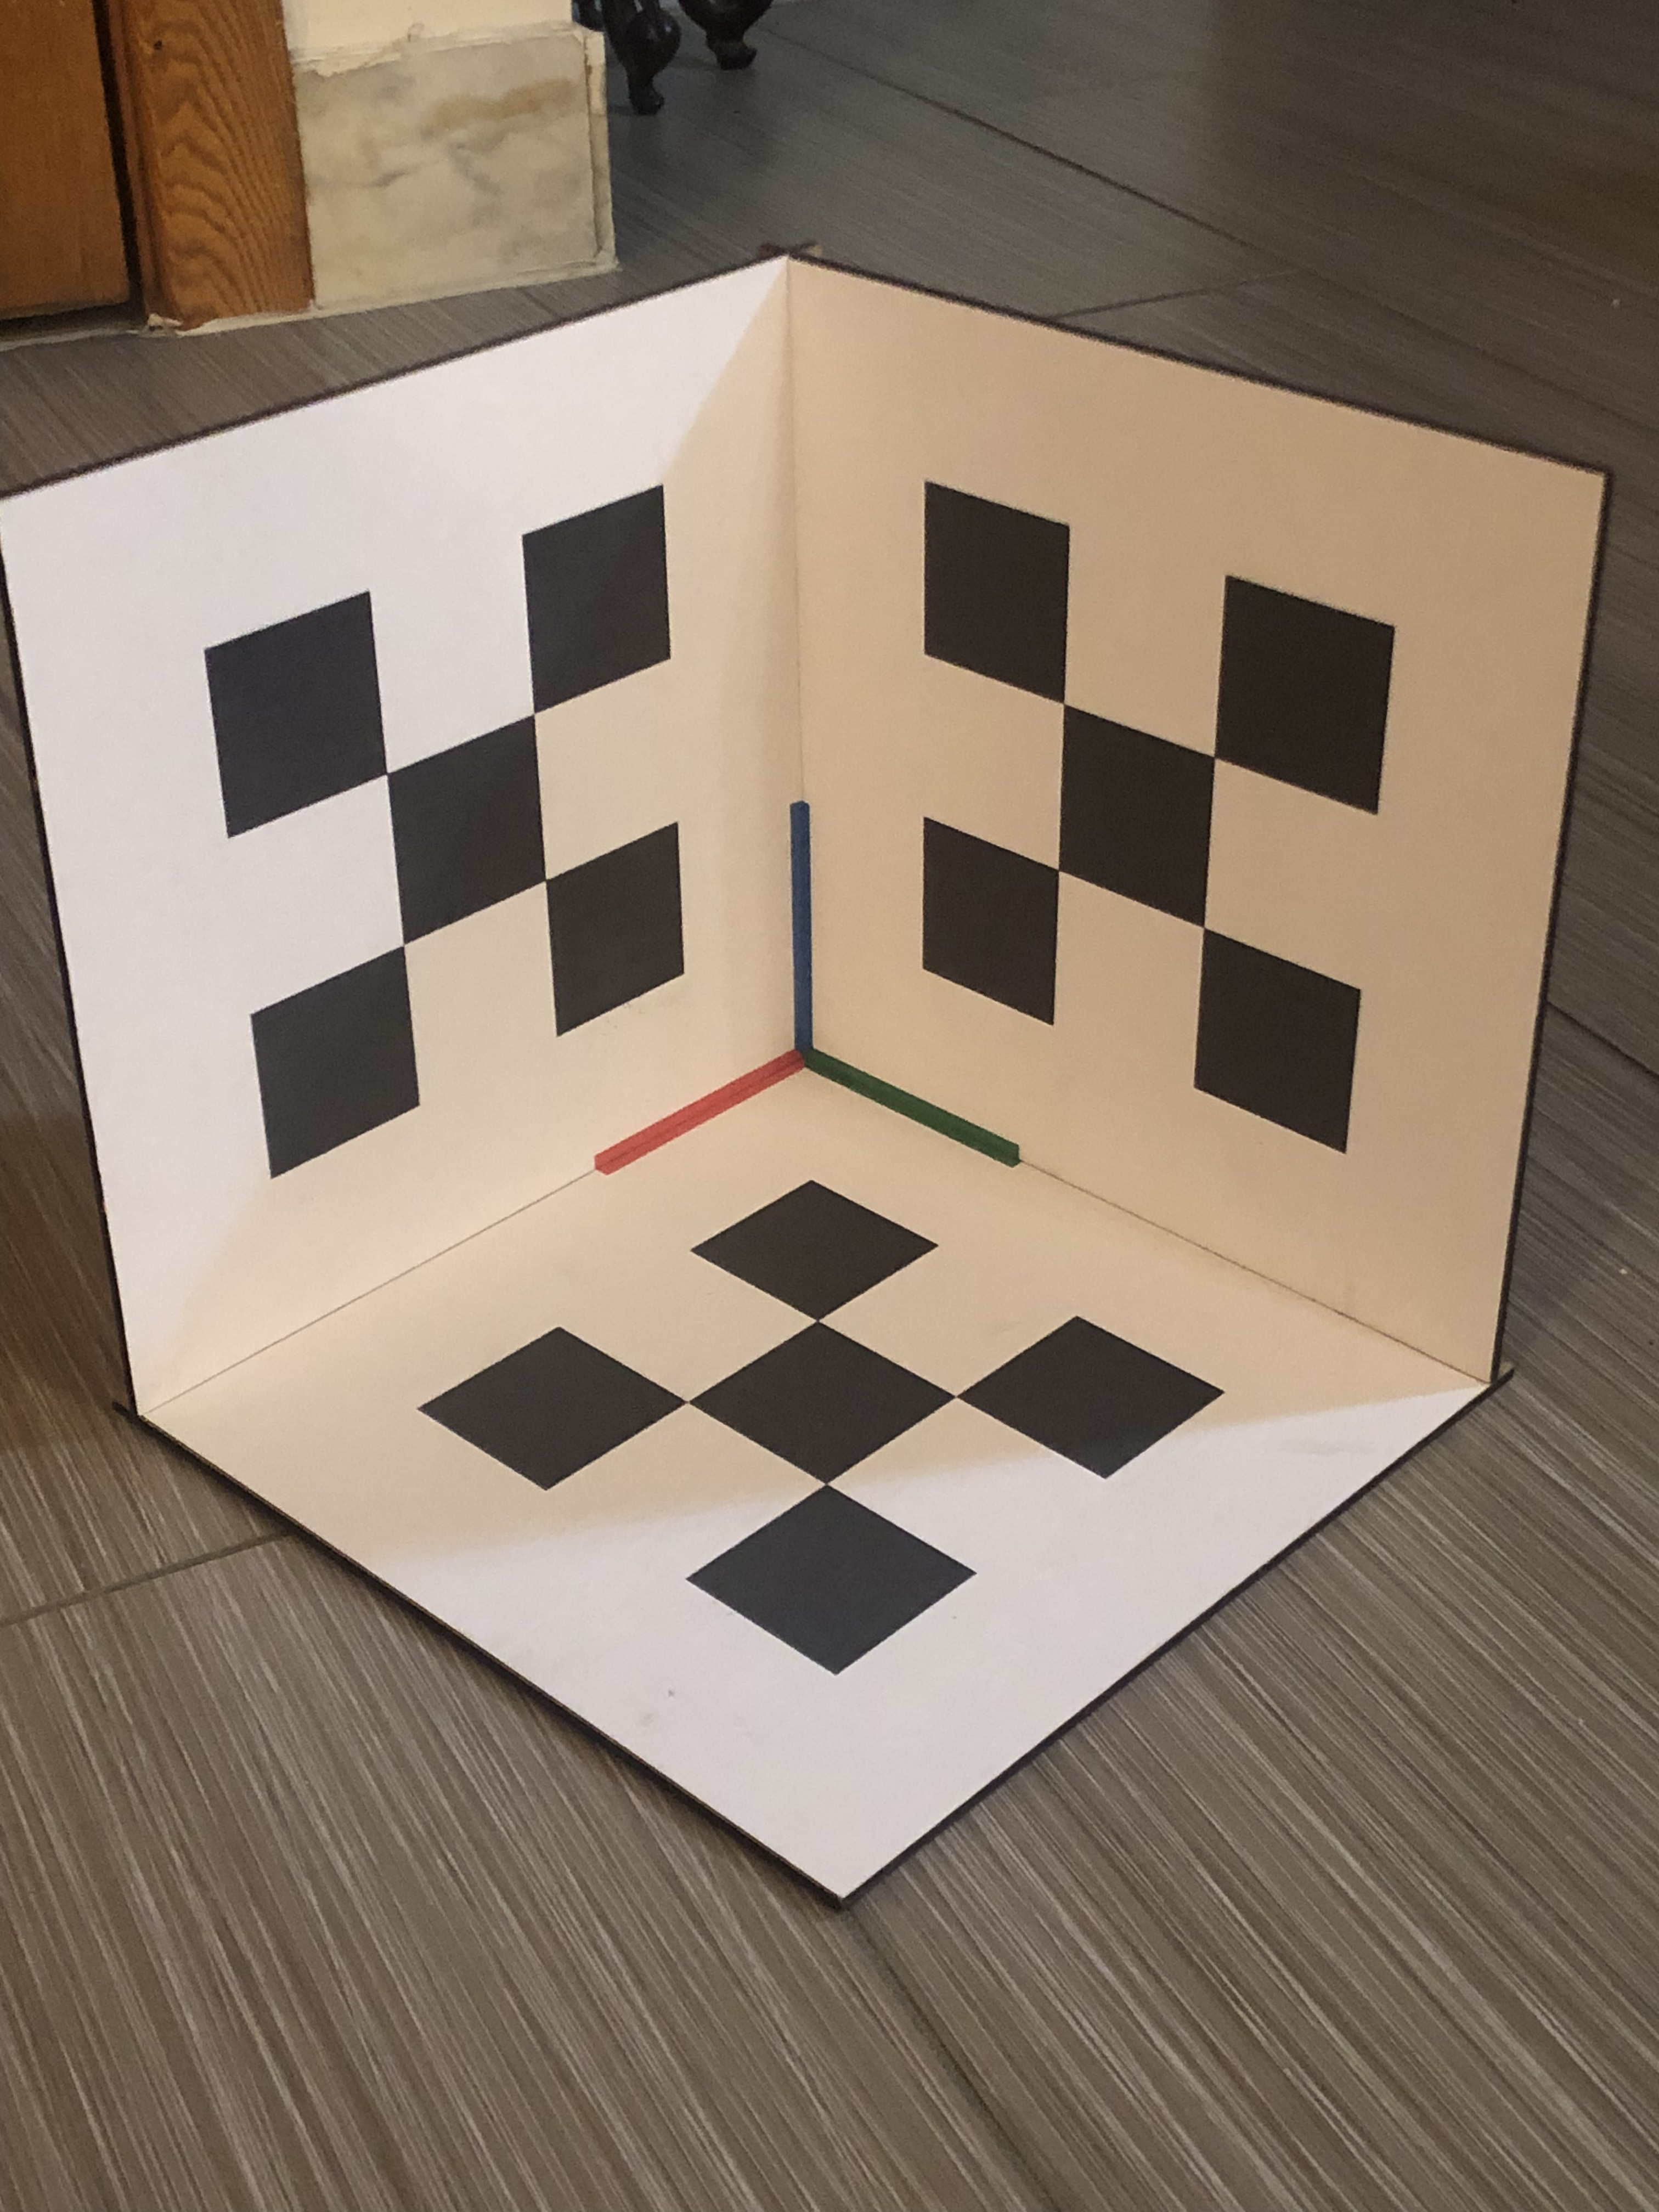
\includegraphics[width=0.45\textwidth]{assets/figures/results/iphone_image}
    \caption{Photograph 1. The photo editing software \emph{GIMP} was used for edge detection, and the coordinates of the calibration points were selected manually. }
\end{figure}



\begin{figure}[H]
    \centering
    \includegraphics[width=0.8\textwidth]{assets/figures/results/iphone_graph}
    \caption{Graph produced by \texttt{Matplotlib} which displays the results of the trial}
\end{figure}

\begin{equation*}
    P =
    \begin{bmatrix}
        \num{-2.5844e-03} & \num{1.7334e-03}  & \num{-4.6719e-04} & \num{6.0581e-01} \\
        \num{4.8240e-04}  & \num{4.4097e-04}  & \num{-3.1337e-03} & \num{7.9559e-01} \\
        \num{-3.3990e-07} & \num{-3.1311e-07} & \num{-2.8179e-07} & \num{4.1340e-04}
    \end{bmatrix}
\end{equation*}

\begin{longtable}{| C{0.15\textwidth} | C{0.30\textwidth} |}
    \caption{Parameters}                \\
    \hline
    Parameter & Value                   \\
    \endfirsthead
    \hline
    \hline
    $f_x$     & $\qty{5590.33}{\pixel}$ \\
    $f_y$     & $\qty{5571.69}{\pixel}$ \\
    \hline
    $c_x$     & $\qty{1595.16}{\pixel}$ \\
    $c_y$     & $\qty{1983.06}{\pixel}$ \\
    \hline
    $\alpha$  & $\qty{38.90}{\degree}$  \\
    $\beta$   & $\qty{29.52}{\degree}$  \\
    $\gamma$  & $\qty{-48.01}{\degree}$ \\
    \hline
    $t_x$     & $\qty{470.72}{\mm}$     \\
    $t_y$     & $\qty{457.63}{\mm}$     \\
    $t_z$     & $\qty{390.74}{\mm}$     \\
\end{longtable}

The reprojection error, $\mu$, was calculated to be $\pm \qty{3.02}{\pixel}$.


\input{sections/applications}
% =================================================================

%TC:ignore
\section*{Acknowledgements}
\addcontentsline{toc}{section}{Acknowledgements}

I am very grateful to my supervisor Mr. Hoteit for his continual guidance and invaluable pieces of advice during the process of writing this extended essay. I would also like to thank Aditya, for aiding me with the creation of some diagrams used.

\clearpage
\pagestyle{backmatter}

\printbibliography[heading=bibintoc]{}

% =================================================================

\clearpage
\begin{appendices}
    \pagestyle{appendices}
    \section{Data}

\input{assets/tables/cal_1}

    \section{Partial Derivatives} \label{sec:partial}

    \input{sections/appendix/lagrangian}
    \section{Eigenvalue and Eigenvector Problem}

which states that for a given matrix $M \in \mathbb{R}^{n \times n}$, determine the eigenvector $x \in \mathbb{R}^n, x \neq 0$ and the eigenvalue $\lambda \in \mathbb{C}$ such that:
\begin{equation*}
    Mx = \lambda x
\end{equation*}


\end{appendices}
%TC:endignore

\end{document} % END

